\newpage
\section{General Convex Problem}

\subsection{Motivation and Definitions}

\subsubsection{Motivation}

\begin{align*}
    &\min f_0(\bx)\\
    \st & f_i(\bx)\le 0,\ i=1,\dots,m\\
    &\bx \in Q \subseteq \R^n
\end{align*}
non-differentiable

\begin{definition}[Interior Point]
    An element $\bx \in C\subset \R^n $ is called an interior point of $C$ if there exists an $\epsilon>0$ for which
    \begin{align*}
        \left\{ \by \left| \norm{\by-\bx}_2\le \epsilon \right. \right\}\subset C
    \end{align*}
\end{definition}
以及另一个 related interior point

\begin{definition}[Open and Closed Set]
    A set $C$ is open if $int\ C=C$, i.e. every point in $C$ is an interior point. A set $C\subset \R^n$ is closed if its complement $\R^n/C=\left\{ \bx \in \R^n |\bx \notin C \right\}$ is open. 
\end{definition}

经常出现不光滑的优化问题. 
\begin{itemize}
    \item max-type functions
    \item 隐式给出问题
\end{itemize}

Denoted by
\begin{align*}
    \dom f=\left\{ \bx\in\R^n : |f(\bx)|<\infty \right\}
\end{align*}
the domain of function $f$. We always assume that $\dom f \ne \emptyset$

\subsubsection{Definition of Convex Function}

\begin{definition}
    A function $f(\bx)$ is called convex, if its domain is convex and $\forall \bx,\by \in \dom\ f$ and $\alpha\in[0,1]$ the following inequality holds
    \begin{align*}
        f(\alpha \bx +(1-\alpha)\by)\le \alpha f(\bx)+(1-\alpha)f(\by)
    \end{align*}
    If this inequality is strict(严格小于), the function is called strictly convex. We call $f$ concave if $-f$ is Convex. 
\end{definition}
之前学的优化都是 gradients, 对于不光滑的, 需要更多的技巧. 


\begin{lemma}[Jensen's Inequality]
    For ang $\bx_1,\dots,\bx_m\in \dom f$ and positive coefficients $\alpha_1, \dots, \alpha_m$ such that 
    \begin{align}
        \sum_{i=1}^m \alpha_i=1,\ \alpha\ge 0,\ i=1,\dots,m \label{eq:512}
    \end{align}
    we have
    \begin{align*}
        f(\sum_{i=1}^m \alpha_i \bx_i)\le \alpha_i f(\bx_i)
    \end{align*}
\end{lemma}

A point $\displaystyle \bx=\sum_{i=1}^m \alpha_i\bx_i$ with positive coefficients $\alpha_i$ satisfying the normalizing condition \ref{eq:512} is called a convex combination(凸组合) of points $\left\{ \bx_i \right\}_{i=1}^m$. 
% \begin{proof}
    
% \end{proof}

\begin{corollary}
    Let $\bx$ be a convex combination of points $\bx_1, \dots, \bx_m$, then
    \begin{align*}
        f(\bx)\le \max_{1\le i\le m}f(\bx_i)
    \end{align*}
\end{corollary}

\begin{corollary}
    Let
    \begin{align*}
        \Delta &= Conv\{ \bx_1,\dots,\bx_m \}\\
        &=\left\{ \left. \bx=\sum_{i=1}^m\alpha_i\bx_i \right|\alpha_i\ge 0,\ \sum_{i=1}^m \alpha_i=1\right\}
    \end{align*}
    $Conv$ means convex combination. 
    
    Then $\displaystyle \max_{\bx\in\Delta}f(\bx)=\max_{1\le i\le m}f(\bx_i)$
\end{corollary}

\begin{theorem}
    A function $f$ is convex iff $\forall \bx, \by \in \dom f$ and $\beta\ge 0$ such that $\by+\beta(\by-\bx)\in\dom f$, we have
    \begin{align*}
        f(\by+\beta(\by-\bx))\ge f(\by)+\beta (f(\by)-f(\bx))
    \end{align*}
\end{theorem}

\begin{theorem}
    A function $f$ is convex iff its epigraph(函数线以上的区域)
    \begin{align*}
        epi(f)=\left\{ (\bx,t)\in \dom f\times \R | t\ge f(\bx) \right\}
    \end{align*}
    is a convex set. 
\end{theorem}

\begin{theorem}
    If a function $f$ is convex, then all level sets(层集)
    \begin{align*}
        \LC_f(\beta)=\left\{ \bx \in \dom f| f(\bx)\le \beta \right\}
    \end{align*}
    are either convex or empty. 
\end{theorem}

\subsubsection{Other Properties}
\begin{definition}
    A function $f$ is called closed and convex if its epigraph is a closed set.
\end{definition}
\begin{theorem}
    If convex function $f$ is closed, then all its level sets are either empty or closed. 
\end{theorem}

% \subsubsection{Examples}
pathological(病态)

\subsection{Operation with Convex Function}
\subsubsection{Invariant Operations}

\begin{definition}[Lower Semicontinuity]
    A function $f$ is lower-semicontinuity at a given vector $\bar\bx$ if for every sequence $\{ \bx_k \}$ converging to $\bar\bx$, we have
    \begin{align*}
        \lim\inf_{k\to\infty} f(\bx_k)\ge f(\bar\bx)
    \end{align*}
    We say that $f$ is lower-semicontinuity over a set $X$ if $f$ is lower-semicontinuity at every $\bx\in X$.
\end{definition}

Note:
\begin{align*}
    \lim\inf_{k\to\infty}\bx_k\iff \lim_{k\to\infty}\left( \inf_{m\ge k}\bx_m \right)
\end{align*}

\begin{theorem}
    For a function $f:\R^n\to\R\cup\{ -\infty,+\infty \}$ the following statements are equivalent
    \begin{enumerate}
        \item $f$ is closed
        \item Every level set of $f$ is closed
        \item $f$ is lower-semicontinuity oevr $\R^n$
    \end{enumerate}
\end{theorem}

\begin{figure}[!htb]
    \centering
    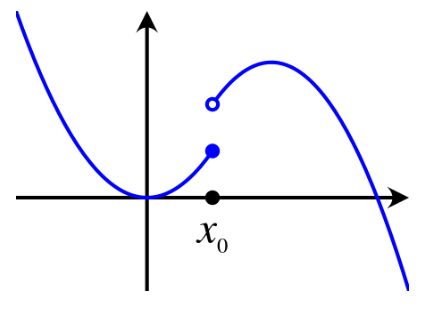
\includegraphics[width=0.309\textwidth]{pic/Opt5/Invariant Operations}
    \caption{$f$}
\end{figure}


Let us describe a set of invariant operations to create more complicated objects. 
\begin{theorem}
    Let function $f_1$ and $f_2$ be closed and convex and let $\beta\ge 0$. Then all functions below are closed and convex:
    \begin{enumerate}
        \item $f(\bx)=\beta f_1(\bx),\ \dom f=\dom f_1$
        \item $f(\bx)=f_1(\bx)+f_2(\bx),\ \dom f=(\dom f_1)\cap (\dom f_2)$
        \item $f(\bx)=\max\{ f_1(\bx),f_2(\bx) \},\ \dom f=(\dom f_1)\cap (\dom f_2)$
    \end{enumerate}
\end{theorem}

The following theorem demonstrates that convexity is an affine-invariant property. 
\begin{theorem}
    Let function $\phi(\by),\ \by\in\R^n$ be convex and closed. Consider a linear operator
    \begin{align*}
        \mathcal{A}(\bx)=A\bx+b: \R^n\to \R^m
    \end{align*}
    Then $f(\bx)=\phi(\mathcal{A}(\bx))$ is a closed and convex function with domain
    \begin{align*}
        \dom f=\{ \bx\in\R^n | \mathcal{A}(\bx)\in \dom \phi \}
    \end{align*}
\end{theorem}

The next theorem is one of the main suppliers of convex functions with implicit structure. 
\begin{theorem}
    Let $\Delta$ be some set and 
    \begin{align*}
        f(\bx)=\sup_{\by}\left\{ \phi(\by,\ \bx)|\by\in\Delta \right\}
    \end{align*}
    Suppose that for any fixed $\by \in \Delta$, the function $\phi(\by,\ \bx)$ is closed and convex in $\bx$. Then $f(\bx)$ is a closed convex function with domain
    \begin{align*}
        \dom f=\left\{\left. \bx\in\bigcap_{\by\in\Delta}\dom \phi(\by,\ \cdot) \right| \exists \gamma : \phi(\by, \bx)\le \gamma,\ \forall \by \in \Delta \right\}
    \end{align*}
\end{theorem}

% \subsubsection{Examples}

\subsection{Continuity and Differentiability}

\subsubsection{Continuity of Convex Function}
\begin{lemma}
    Let $f$ be convex and $\bx_0\in int(\dom f)$. Then $f$ is locally upper bounded at $\bx_0$. 
\end{lemma}

% proof use corollary V.6

\begin{theorem}
    Let $f$ be convex and $\bx_0\in int(\dom f)$. Then $f$ is locally Lipschitz continuous at $\bx_0$. 
\end{theorem}
Remark: 构造 $\bm{z}$ 没有超出领域, $\by$ 是 $\bx_0$ 与 $\bm{z}$ 的凸组合.

\subsubsection{Differentiability of Convex Function}

\begin{definition}
    Let $\bx\in\dom f$. We call $f$ differentiable in a direction $p$ at point $\bx$ if the following limit exists
    \begin{align*}
        f'(\bx;\bm{p})=\lim_{\alpha \downarrow 0}\frac{1}{\alpha}\left[f(\bx+\alpha\bm p)-f(\bx)\right]
    \end{align*}
    The value $f'(\bx;\bm p)$ is called the directional derivative of $f$ at $\bx$. 
\end{definition}

\begin{theorem}
    Convex $f$ is differentiable in any direction at any interior point of its domain. 
\end{theorem}

\begin{lemma}
    Let $f$ be a convex function and $\bx\in int (\dom f)$. Then $f'(\bx;\bm p)$ is a convex function of $\bm p$, which is homogeneous of degree 1. For any $\by\in \dom f$ we have
    \begin{align*}
        f(\by)\ge f(\bx)+f'(\bx; \by-\bx)
    \end{align*}
\end{lemma}

\subsection{Separation Theorem}

\subsubsection{Projection}

\begin{definition}[Hyperplane]
    Let $Q$ be a convex set. We say that hyperplane
    \begin{align*}
        \mathcal{H}(\bm g,\gamma)=\left\{ \bx \in \R^n| \braket{\bm g, \bx}=\gamma \right\},\ \bm g\ne 0
    \end{align*}
    is supporting to $Q$ if any $\bx \in Q$ satisfies inequality $\braket{\bm g, \bx}\le \gamma$. 

    We say that the hyperplane $\mathcal{H}(\bm g, \gamma)$ separates a point $\bx_0$ from $Q$ if 
    \begin{align}
        \braket{\bm g, \bx}\le \gamma \le \braket{\bm g, \bx_0} \label{eq:528}
    \end{align}
    $\forall \bx\in Q$. If the second inequality in \ref{eq:528} is strict, we call the separation strict. 
\end{definition}

\begin{definition}[Projection]
    Let $Q$ be a closed set and $\bx_0\in\R^n$. Denote 
    \begin{align*}
        \pi_Q(\bx_0)=\argmin\left\{ \norm{\bx-\bx_0}:\bx \in Q \right\}
    \end{align*}
    We call $\pi_Q(\bx_0)$ the projection of point $\bx_0$ onto the set $Q$. 
\end{definition}

\begin{theorem}
    If $Q$ is a convex set, then there exists a unique projection $\pi_Q(\bx_0)$
\end{theorem}
Remark: It's clear that $\pi_Q(\bx_0)=\bx_0 \iff \bx_0\in Q$. 

\begin{lemma}
    Let $Q$ be a closed and convex set and $\bx_0\notin Q$. Then $\forall \bx\in Q$, we have
    \begin{align*}
        \braket{\pi_Q(\bx_0)-\bx_0, \bx-\pi_Q(\bx_0)}\ge 0
    \end{align*}
\end{lemma}
%TODO 示意图 
从 $\bx$ 到 $\pi_Q(\bx_0)$ 的向量与 从 $\pi_Q(\bx_0)$ 到 $\bx_0$ 的向量 的夹角是锐角. 
\begin{lemma}
    $\forall \bx\in Q$, we have
    \begin{align*}
        \norm{\bx-\pi_Q(\bx_0)}^2+\norm{\pi_Q(\bx_0)-\bx_0}^2\le \norm{\bx-\bx_0}^2
    \end{align*}
\end{lemma}

\subsubsection{Main Theorems}
\begin{theorem}
    Let $Q$ be a closed set and $\bx_0\notin Q$. Then there exists a hyperplane $\mathcal{H}(\bm g, \gamma)$, which strictly separates $\bx_0$ from $Q$. Namely, we can take
    \begin{align*}
        \bm g&=\bx_0-\pi_Q(\bx_0)\ne 0\\
        \gamma&=\braket{\bx_0-\pi_Q(\bx_0), \pi_Q(\bx_0)}
    \end{align*}
\end{theorem}

$\psi(\bm g)=\sup\left\{ \braket{\bm g, \bx}|\bx \in Q \right\}$

\begin{corollary}
    Let $Q_1$ and $Q_2$ be two closed convex sets.
    \begin{enumerate}
        \item If $\forall \bm g\in \dom \psi_{Q_2}$ we have $\psi_{Q_1}(\bm g)\le \psi_{Q_2}(\bm g)$, then $Q_1\subseteq Q_2$. 
        \item Let $\dom \psi_{Q_1}=\dom \psi_{Q_2}$ and $\forall \bm g\in \dom \psi_{Q_1}$, we have $\psi_{Q_1}(\bm g)=\psi_{Q_2}(\bm g)$. Then $Q_1\equiv Q_2$. 
    \end{enumerate}
\end{corollary}

\begin{theorem}
    Let $Q$ be a closed and convex set, and $\bx_0$ belong to boundary of set $Q$. Then there exists a hyperplane $\mathcal{H}(\bm g, \gamma)$, supporting to $Q$ and passing through $\bx_0$. 

    Such a vector $\bm g$ is called supporting to $Q$ at $\bx_0$. 
\end{theorem}

\subsection{Subgradient}

\subsubsection{Definition of Subgradient}

\begin{definition}
    Let $f$ be a convex function. A vector $\bm g$ is called a subgradient of function $f$ at point $\bx_0\in\dom f$ if for any $\bx\in\dom f$, we have
    \begin{align*}
        f(\bx)\ge f(\bx_0)+\braket{\bm g ,\bx-\bx_0}
    \end{align*}
    The set of all subgradient of $f$ at $\bx_0$, is called the subdifferential of function $f$ at point $\bx_0$. 
\end{definition}

Subgradient and Convexity
\begin{lemma}
    Let for any $\bx\in\dom f$ subdifferential $\partial f(\bx)$ be nonempty. Then $f$ is a convex function. 
\end{lemma}

\begin{theorem}
    Let $f$ be closed and convex and $\bx_0\in int(\dom f)$. Then $\partial f(\bx_0)$ is a nonempty bounded set. 
\end{theorem}

\begin{theorem}
    Let $f$ be a closed convex function. For any $\bx_0\in int(\dom f)$ and  $\bm p\in\R^n$, we have
    \begin{align*}
        f'(\bx_0;\bm p)=\max\{ \braket{\bm g, \bm p}|\bm g\in\partial f(\bx_0) \}
    \end{align*}
\end{theorem}

\subsubsection{Properties of Subgradient}

\begin{theorem}
    We have 
    \begin{align*}
        f(\bx^*)=\min_{\bx\in\dom f}f(\bx)\iff 0\in \partial f(\bx^*)
    \end{align*}
\end{theorem}

\begin{theorem}
    For any $\bx_0\in\dom f$, all vector $\bm g\in\partial f(\bx_0)$ are supporting to the level set $\mathcal{L}_f(f(\bx_0))$:
    \begin{align*}
        \braket{\bm g, \bx_0-\bx}&\ge 0\\
        \forall \bx\in \mathcal{L}_f(f(\bx_0))&\equiv \{ \bx\in\dom f:f(\bx)\le f(\bx_0) \}
    \end{align*}
\end{theorem}

\begin{corollary}
    Let $Q\subseteq \dom f$ be a closed convex set, $\bx_0\in Q$ and 
    \begin{align*}
        \bx x^*=\argmin \{ f(\bx)|\bx\in Q \}
    \end{align*}
    Then $\forall \bm g \in \partial f(\bx_0)$, we have $\braket{\bm g, \bx_0-\bx^*}\ge 0$. 
\end{corollary}

\subsubsection{Rules for Computing}
\begin{lemma}
    Let $f$ be closed and convex. Assume that it's differentiable on its domain. Then
    \begin{align*}
        \partial f(\bx)=\left\{ \nabla f(\bx) \right\}
    \end{align*}
    $\forall \bx\in int(\dom f)$
\end{lemma}

\begin{lemma}
    Let $f(\by)$ be closed and convex with $\dom f\subseteq \R^m$. Consider a linear operator 
    \begin{align*}
        \mathcal{A}(\bx)=A\bx+\bm b: \R^n\to \R^m
    \end{align*}
    Then $\phi(\bx)=f(\mathcal{A}(\bx))$ is closed convex function with domain $\dom \phi=\{ \bx|\mathcal{A}(\bx)\in \dom f \}$. $\forall \bx\in int(\dom \phi)$, we have
    \begin{align*}
        \partial \phi(\bx)=A^{\top} \partial f(\mathcal{A}(\bx))
    \end{align*}
\end{lemma}

\begin{lemma}
    Let $f_1(\bx)$ and $f_2(\bx)$ be closed convex function and $\alpha_1, \alpha_2\ge 0$. Then function $f(\bx)=\alpha_1f_1(\bx)+\alpha_2f_2(\bx)$ is closed and convex and
    \begin{align*}
        \partial f(\bx)=\alpha_1\partial f_1(\bx)+\alpha_2\partial f_2(\bx)
    \end{align*}
    $\forall \bx \in int(\dom f)=int(\dom f_1)\cap int(\dom f_2)$
\end{lemma}

\begin{lemma}
    Let functions $f_i(\bx),\ i=1,\dots,m$ be closed and convex. Then function
    \begin{align*}
        f(\bx)=\max_{1\le i\le m}f_i(\bx)
    \end{align*}
    is also closed and convex. $\displaystyle \forall \bx \in int(\dom f)=\bigcap_{i=1}^m int(\dom f_i)$, we have
    \begin{align*}
        \partial f(\bx)=Conv\{ \partial f_i(\bx)|i\in I(\bx) \}
    \end{align*}
    where $I(\bx)=\{ i: f_i(\bx)=f(\bx) \}$
\end{lemma}

\begin{lemma}
    Let $\Delta$ be a set and $f(\bx)=\sup\{ \phi(\by,\bx)|\by\in\Delta \}$. Suppose that for any fixed $\by\in\Delta$, the function $\phi(\by,\bx)$ is closed and convex in $\bx$. Then $f(\bx)$ is closed convex. 

    Moreover, for any $\bx$ from 
    \begin{align*}
        \dom f=\{ \bx\in\R^n|\exists \gamma:\phi(\by, \bx)\le \gamma,\ \forall \by \in \Delta \}
    \end{align*}
    we have
    \begin{align*}
        \partial f(\bx)\supseteq Conv\{ \partial \phi_{\bx}(\by,\bx)|\by\in I(\bx) \}
    \end{align*}
    where $I(\bx)=\{ \by|\phi(\by,\bx)=f(\bx) \}$
\end{lemma}

\begin{theorem}
    Let $\norm{\cdot}$ be a vector norm in $\R^n$, then 
    \begin{align*}
        \partial \norm{\cdot}=\left\{ V(\bx) \triangleq \left\{ \bm v\in\R^n|\braket{\bm v,\bx}=\norm{\bx},\ \norm{\bm v}\le 1 \right\} \right\}
    \end{align*}
    where $\norm{\bm v}_*$ is the dual norm of $\norm{\cdot}$, defined as
    \begin{align*}
        \norm{\bm v}_* \triangleq \sup_{\norm{\bm u}\le 1}\braket{\bx, \bm u}
    \end{align*}
\end{theorem}


\subsection{General Lower Complexity Bounds}

\subsubsection{Problem Class}
We have 
\begin{align*}
    \min_{\bx\in\R^n}f(\bx)
\end{align*}

\begin{table}[H]%TODO 
    \centering
    \caption{Problem Class}
    \begin{tabular}[c]{cc}\toprule
        Model & \\ \cmidrule{1-1}
        Oracle & \\ \cmidrule{1-1}
        Approximate solution & \\ \cmidrule{1-1}
        Method & \\ 
        \bottomrule
    \end{tabular}
\end{table}


\subsubsection{Resisting Oracle}
Special Function family

Let us fix some constant $\mu>0$ and $\gamma>0$, 
\begin{align*}
    f_k(\bx)=\gamma \max_{1\le i\le k}\bx^{(i)}+\frac{\mu}{2}\norm{\bx}^2,\ k=1,\dots,n
\end{align*}

\begin{align*}
    \partial f_k(\bx)&=\mu\bx+\gamma Conv\{ e_i|i\in I(\bx) \}\\
    I(\bx)&=\left\{ 1\le j\le k, \bx^{(j)}=\max_{1\le i\le k}\bx^{(i)} \right\}
\end{align*}

\begin{enumerate}
    \item Loacl Lipschitz Continuity of $f_k$
    \subitem Therefore $\forall \bx, \by\in B_2(0,\rho),\rho>0$, and $g_k(\by)\in\partial f_k(\by)$, we have
    \begin{align*}
        f_k(\by)-f_k(\bx)&\le \braket{g_k(\by), \by-\bx}\\
        &\le \norm{g_k(\by)}\cdot \norm{\by-\bx}\\
        &\le (\mu\rho+\gamma)\norm{\by-\bx}
    \end{align*}
    Thus $f_k$ is Lipschitz continuous on $B_2(0,\rho)$ with Lipschitz constant
    \begin{align*}
        M=\mu\rho+\gamma
    \end{align*}
    \item minimum of $f_k$
    \subitem Further, consider the point $\bx_k^*$ with the coordinates
    \begin{align*}
        \left( \bx_k^* \right)^{(i)}=\left\{ \begin{array}{ll}
            -\frac{\gamma}{\mu k}& 1\le i\le k\\
            0 & K=1\le i\le n
        \end{array} \right.
    \end{align*}
    It's easy to check that $0\in\partial f_k\left( \bx_k^* \right)$, and therefore $\bx_k^*$ is the minimum of $f_k(\bx)$. Note that
    \begin{align*}
        R_k&=\norm{\bx_k^*}=\frac{\gamma}{\mu \sqrt{k}}\\
        f_k^*&=-\frac{\gamma^2}{\mu k}+\frac{\mu}{2}R_k^2=-\frac{\gamma^2}{2\mu k}
    \end{align*}
    \item The subgradient of $f_k$
    \subitem %TODO
    \item Characteristic of $\bx_{i+1}$ generated by resisting oracle
    \subitem Let us choose starting point $\bx_0=0$. Denote
    \begin{align*}
        \R^{p,n}=\left\{ \bx\in\R^n | \bx^{(i)}=0,p+1\le i\le n \right\}
    \end{align*}
    %TODO 
\end{enumerate}

\subsubsection{Lower Bound}

\begin{theorem}
    For nay class $\mathcal{P}(\bx_0, R, M)$ and any $k$, $0\le k\le n-1$, there exists a function $f\in \mathcal{P}(\bx_0, R, M)$ such that
    \begin{align*}
        \bx_k\in\bx_0 +Lin\left\{ g(\bx_0),\dots,g(\bx_{k-1}) \right\}
    \end{align*}
    for any optimization scheme, which generates a  sequence $\left\{ \bx_k \right\}$ satisfying the condition
    \begin{align*}
        f(\bx_k)-f^*\ge \frac{MR}{2(1+\sqrt{k+1})}
    \end{align*}
\end{theorem}

\subsection{Subgradient Method}
\subsubsection{property of Subgradient}
\begin{align*}
    \min \left\{ f(\bx)|\bx\in Q \right\}
\end{align*}

\begin{align*}
    \braket{g(\bx), \bx-\bx^*}\ge 0
\end{align*}
\begin{itemize}
    \item The distance between $\bx$ and $\bx^*$ is decreasing in the direction $-g(\bx)$
    \item In equality (4) cuts $\R^n$ into two galf-spaces. Only one of them contains $\bx^*$
\end{itemize}

\subsubsection{Main Lemma}
Let us fix some $\bar{\bx}\in\R^n$. For $\bx\in\R^n$ with $g(\bx)\ne 0$ define
\begin{align*}
    v_f(\bar{\bx}, \bx)=\frac{1}{\norm{g(\bx)}}\braket{g(\bx), \bx-\bar{\bx}}
\end{align*}
If $g(\bx)=0$, then define $v_f(\bar{\bx}, \bx)=0$. Clearly, $v_f(\bar{\bx}, \bx)\le \norm{\bx-\bar{\bx}}$


%TODO

Let us introduce a function that measures the variation of function $f$ with respect to the point $\bar{\bx}$. For $t\ge 0$, define
\begin{align*}
    \omega_f(\bar{\bx};t)=\max\left\{ f(\bx)-f(\bar{\bx})|\norm{\bx-\bar{\bx}}\le t \right\}
\end{align*}
If $t<0$, we set $\omega_f(\bar{\bx};t)=0$. Clearly, the function $\omega_f$ possesses the following Properties:
\begin{enumerate}
    \item For all $t<0$, $\omega_f(\bar{\bx};0)=0$
    \item $\omega_f(\bar{\bx};t)$ is a nondecreasing function of $t$, $t\in\R^1$
    \item $f(\bx)-f(\bar{\bx})\le \omega_f(\bar{\bx};\norm{\bx-\bar{\bx}})$
\end{enumerate}

\begin{lemma}
    For any $\bx\in\R^n$, we have
    \begin{align*}
        f(\bx)-f(\bar{\bx})\le \omega_f(\bar{\bx};v_f(\bar{\bx},\bx))
    \end{align*}
    If $f(\bx)$ is Lipschitz continuous on $B_2(\bar{\bx}, R)$ with some $M$, then
    \begin{align*}
        f(\bx)-f(\bar{\bx})\le M(v_f(\bar{\bx}, \bx))_+
    \end{align*}
    $\forall \bx\in\R^n$ with $\omega_f(\bar{\bx}; \bx)\le \R$
\end{lemma}

\begin{definition}
    Let $\left\{ \bx_i \right\}_{i=0}^\infty$ be a sequence in $Q$. Define
    \begin{align*}
        S_k=\left\{ \bx\in Q|\braket{g(\bx_i), \bx_i-\bx}\ge 0,i=0,\dots,k \right\}
    \end{align*}
    We call this set the location set of problem (3) generated by sequence $\left\{ \bx_i \right\}_{i=0}^\infty$.  
\end{definition}
Note that in view of inequality (4) $\forall k\ge 0$, we have $\bx^*\in S_k$. Denote
\begin{align*}
    v_i&=v_f(\bx^*;\bx_i)\ge 0\\
    v_k^*&=\min_{0\le i\le k}v_i
\end{align*}
Thus
\begin{align*}
    v_k^*=\max\left\{ r|\braket{g(\bx_i), \bx_i-\bx}\ge0,i=0,\dots,k,\forall \bx\in B_2(\bx^*,r ) \right\}
\end{align*}

\begin{lemma}
    Let $\displaystyle f_k^*=\min_{0\le i\le k}f(\bx_i)$. Then $f_k^*-f^*\le \omega_f(\bx^*;v_k^*)$
\end{lemma}

\subsubsection{Scheme for Non-smooth Problem}

%TODO

\subsubsection{Main Theorem}
\begin{theorem}
    Let $f$ be Lipschitz continuous on $B_2(\bx^*, R)$ with constant $M$ and $\bx_0\in B(\bx^*, R)$. Then
    \begin{align*}
        f_k^*-f^*\le M\frac{R^2+\sum_{i=0}^kh_i^2}{2\sum_{i=0}^kh_i}
    \end{align*}
\end{theorem}


\subsection{Frank-Wolfe Algorithm}
\subsubsection{Problems}

\begin{algorithm}[H]
    \caption{Frank-Wolfe Algorithm}
    \begin{algorithmic}
        \State %TODO
    \end{algorithmic}
\end{algorithm}


\subsubsection{Examples}


\subsubsection{Convergence Theory}
\begin{definition}
    We will say that $\bx^*\in\mathcal{D}$ is a stationary point if
    \begin{align*}
        \braket{\nabla f(\bx^*), \bx-\bx^*}\ge 0
    \end{align*}
    $\forall\bx\in\mathcal{D}$
\end{definition}

\begin{definition}
    We denote by $g_k$ the Frank-Wolfe gap, defined as
    \begin{align*}
        g_k\equiv \braket{\nabla f(\bx_k), \bx-\bm s_k}
    \end{align*}
\end{definition}

\begin{lemma}
    
\end{lemma}